\chapter{Generative Adversarial Networks - Améliorations}


\section{Apprentissage par Mini-Batch}
\subsection{Principe}
L'apprentissage par Batch consiste à apprendre sur l'ensemble du batch d'apprentissage avant de mettre à jour chaque réseau, et de réitérer l'apprentissage à chaque itération sur l'ensemble du batch d'apprentissage.

On calcule successivement la rétropropagation pour chaque image, on somme l'erreur sur l'ensemble des images et on applique la mise à jour du réseau avec la somme des erreurs. On obtient donc une moyenne des directions de propagation afin d'effectuer la mise à jour.

Certaines bases d'apprentissage étant très grandes - soixante mille avec MNIST par exemple -, on va préférer à l'apprentissage par batch, l'apprentissage par Mini-batch. 
On sélectionne aléatoirement parmi la base d'apprentissage et de tests un nombre plus petit d'éléments.
\subsection{Implémentation}
\paragraph{Mise à jour des poids}
Afin de pouvoir effectuer la rétro-propagation uniquement à la fin de l'itération du minibatch, nous avons simplement 

\paragraph{Sets d'apprentissage et de tests. plus petits}
Dans le cas de MNIST, les chiffres du début de la bdd étant plus simple, nous avons afin d'obtenir de meilleurs résultats parfois effectué une sélection aléatoire sur uniquement une première partie des 60000 images d'apprentissage (cf argument \textit{labelTrainSize}) et des 10000 images de tests (cf argument \textit{labelTestSize}.

\subsection{Résultats}
Notre équipe a obtenu des résultats peu convaincants, et très différents des résultats du groupe Salamandre 
Globalement, l'apprentissage s'effectue légèrement plus rapidement pour un même nombre d'itérations, au prix d'une augmentation du temps de calcul par itération (proportionnel selon la taille des batch). Cette technique a donc été abandonnée.
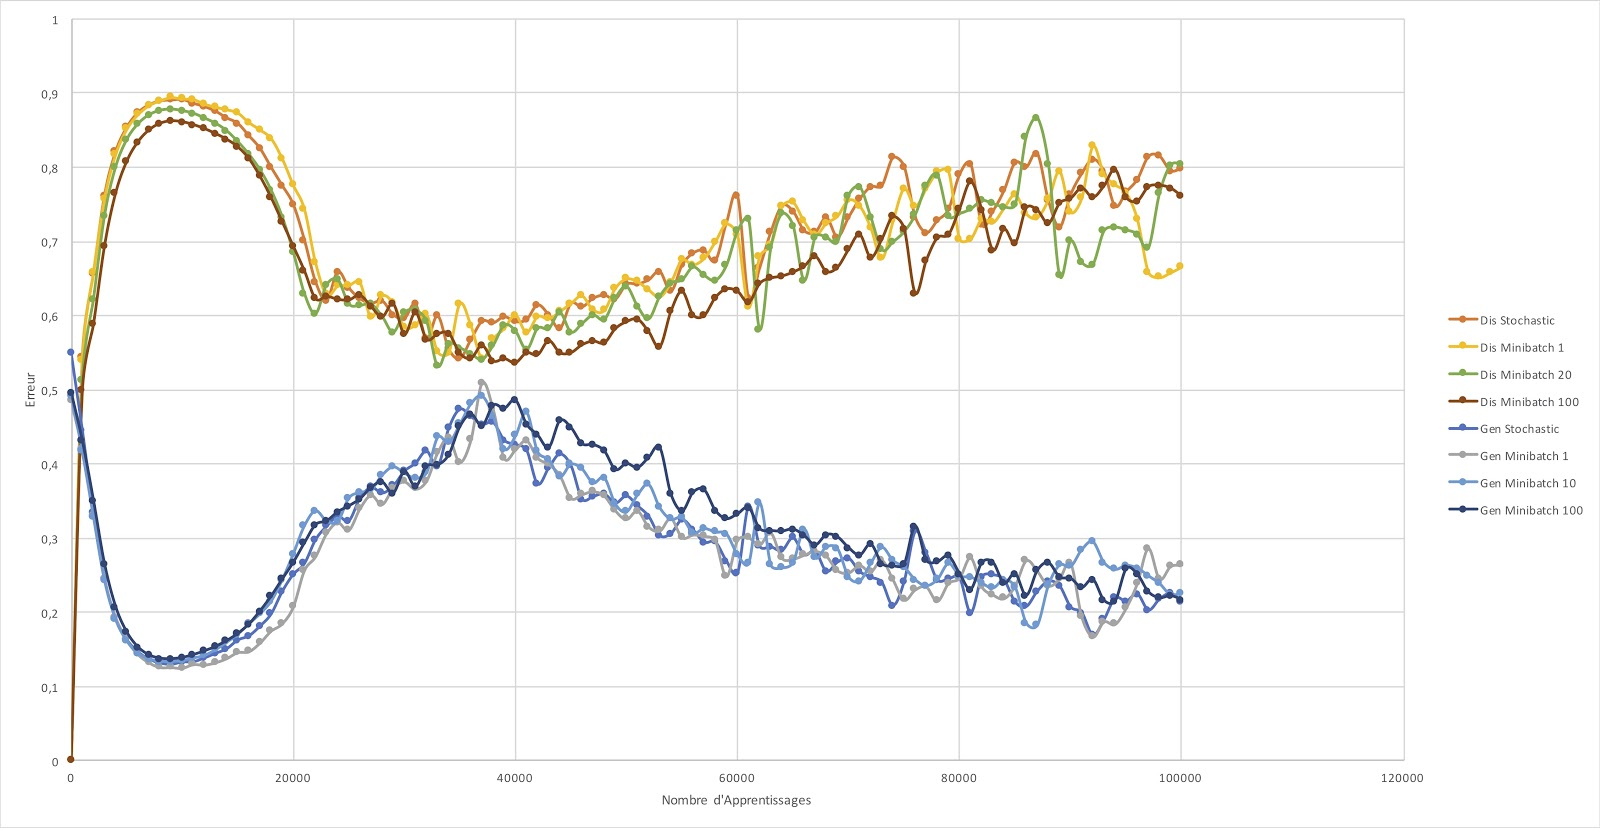
\includegraphics[width=1.5\textwidth]{images/08-gan_ameliorations_resultats_1.jpg}

\section{Algorithmes de pas d'apprentissage adaptatif}
\subsection{Principe}
L'objectif de ces algorithmes est de paramétrer au mieux la convergence de la distribution représentée par notre réseau vers la distribution $p_data$. Le pas adaptatif n'est alors plus constant; il varie en fonction du gradient des étapes d'apprentissage précédentes, de manière plus ou moins évoluée selon les algorithmes.

L'objectif est ainsi de faire évoluer le pas en fonction des erreurs, selon diverses formules. Deux méthodes de pas adaptatifs ont été utilisées : RMSprop et Adam. Nous en présentons ici d'autres.

\subsection{Adagrad}

Cette première méthode de descente adaptative suit les équations suivantes :

\begin{equation}
\begin{aligned}
g_{t+1} = g_t + (\frac{\partial J}{\partial W})^2 \\
W_{t+1} = W_t - \dfrac{\eta}{\sqrt{g_{t+1}} + \epsilon}\frac{\partial J}{\partial W}
\end{aligned}
\end{equation} 

Adagrad n'a pas été implémenté en raison des piètres performances annoncées\textsuperscript{[ref nécessaire])}. En effet, g est strictement croissante, étant incrémenté à chaque itération de $(\frac{\partial J}{\partial W})^2$ . Les réseaux apprenant sur un grand nombre d'itération, le coefficient $g_{t}$ devient rapidement très important, et le pas en $\dfrac{1}{\sqrt{g_{t+1}}}$ devient rapidement négligeable. Les performances de cet algorithme sont donc assez faibles.

\subsection{RMSprop}

La RMSProp permet de résoudre ce problème. En effet, on a un décroissance exponentielle de l'influence de l'erreur dans le temps grâce au coefficient $\gamma$ . Ainsi, l'influence des anciennes valeurs de $(\frac{\partial J}{\partial W})^2$ décroit exponentiellement, les erreurs les plus récentes sont donc les plus influentes sur le pas.

\begin{equation} 
\begin{aligned}
g_{t+1} = \gamma g_t + (1-\gamma)(\frac{\partial J}{\partial W})^2 \\
W_{t+1} = W_t - \dfrac{\eta}{\sqrt{g_{t+1}} + \epsilon}\frac{\partial J}{\partial W}
\end{aligned}
\end{equation} 

\subsection{Adam}
[formule]
Adam est considéré comme plus performante que RMSprop
\subsection{Utilisation}

L’utilisation d’Adam pour le générateur et de RMSProp pour le discriminateur (ayant
comme but d'entraîner mieux le générateur) semble fonctionner bien. La qualité des images
est plus variable (le générateur produit des images laides et belles).
En revanche, l'utilisation de RMSProp pour le générateur et d'Adam pour le discriminateur ne fonctionne pas. Cela corrobore les résultats présentés par d'autres \textsuperscript{[ref nécessaire : rapport appartement + autre ref]}



\section{Réseaux à convolution}

\section{Echanges avec Giuseppe Valenzise}
maître de conférences au laboratoire L2S de CentraleSupélec, spécialiste en Visual Quality Assessment.

